\chapter{Template}
\label{sec:template}

\section{Instructions}

\begin{description}
\item[\textcolor{green}{Author}] Author of the approaches description  \todo{Name -  Company}
\item[\textcolor{blue}{Assessor 1}] First assessor of the approaches \todo{Name - Company}
\item[\textcolor{magenta}{Assessor 2}] Second assessor of the approaches \todo{Name - Company}
\end{description}

In the sequel, main text is under the responsibilities of the author.

\begin{author_comment}
Author can add comments using this format at any place.
\end{author_comment}

\begin{assessor1}
First assessor can add comments using this format at any place.
\end{assessor1}

\begin{assessor2}
Second assessor can add comments using this format at any place.
\end{assessor2}

When a note is required, please follow this list :
\begin{description}
\item[0] not recommended, not adapted, rejected
\item[1] weakly recommended, adapted after major improvements, weakly rejected
\item[2] recommended, adapted (with light improvements if necessary)  weakly accepted
\item[3] highly recommended, well adapted,strongly accepted
\item[*] difficult to evaluate with a note (please add a comment under the table)
\end{description}

All the notes can be commented under each table.

\section{Presentation}

This section gives a quick presentation of the approach and the tool.

\begin{description}
\item[Name] \todo{Name of the approach and the tool}
\item[Web site] \todo{if available, how to  find information}
\item[Licence] \todo{Kind of licence}
\end{description}

\paragraph{Abstract} Short abstract on the approach and tool (10 lines max)

\paragraph{Publications} Short list of publications on the approach (5 max)


For which activities are dedicaded the means or tools (give a note from 0 to  3) :

\begin{tabular}{|l | c | c | c | c|}
\hline
& \textcolor{green}{Author} & \textcolor{blue}{Assessor 1} & \textcolor{magenta}{Assessor 2} & Total \\
\hline 
Verification & & & &  \\
\hline
Validation & & & & \\
\hline
Safety analysis & & & & \\
\hline
Data, function or requirement management & & & & \\
\hline
Model or code transformation & & & & \\
\hline
\end{tabular}

According the results of this table, some of the following sections can be skipped.

\section{Common criteria on secondary means and tools}
\label{common}
This section discusses the common criteria of the means and tools according to the project requirements on tools and the results of T7.1.

\subsection{Project and WP2 requirements}

According WP2 requirements, give a note for characteristics of the use of the tool (from 0 to 3) :

\begin{tabular}{|l | c | c | c | c|}
\hline
& \textcolor{green}{Author} & \textcolor{blue}{Assessor 1} & \textcolor{magenta}{Assessor 2} & Total \\
\hline 
Open Source (D2.6-02-074) & & & &  \\
\hline 
Portability to operating systems (D2.6-02-075) & & & &  \\
\hline
Cooperation of tools (D2.6-02-076) & & & &  \\
\hline
Robustness (D2.6-02-078) & & & & \\
\hline
Modularity (D2.6-02-078.1) & & & & \\
\hline
Documentation management (D2.6-02-078.02) & & & & \\
\hline
Distributed software development (D2.6-02-078.03)  & & & & \\
\hline
Simultaneous multi-users (D2.6-02-078.04)   & & & & \\
\hline
Issue tracking (D2.6-02-078.05) & & & & \\
\hline
Differences between models (D2.6-02-078.06) & & & & \\
\hline
Version management (D2.6-02-078.07) & & & & \\
\hline
Concurrent version development (D2.6-02-078.08) & & & & \\
\hline
Model-based version control (D2.6-02-078.09) & & & & \\
\hline
Role traceability (D2.6-02-078.10) & & & & \\
\hline
Safety version traceability (D2.6-02-078.11) & & & & \\
\hline
Model traceability (D2.6-02-079) & & & & \\
\hline
Tool chain integration & & & & \\
\hline
Scalability & & & & \\
\hline
\end{tabular}

\subsection{Certifiability}

This section discusses how the tool can be classified according EN50128 requirements (D2.6-02-085).


\begin{tabular}{|l | c | c | c | c|}
\hline
& \textcolor{green}{Author} & \textcolor{blue}{Assessor 1} & \textcolor{magenta}{Assessor 2} & Total \\
\hline 
Tool manual (D.2.6-01-42.02) & & & &  \\
\hline
Proof of correctness (D.2.6-01-42.03)   & & & & \\
\hline
Existing industrial  usage  & & & & \\
\hline
Model verification & & & & \\
\hline
Test generation & & & & \\
\hline
Simulation, execution, debugging & & & & \\
\hline
Formal proof & & & & \\
\hline
\end{tabular}

\paragraph{Other elements for tool certification}


\subsection{Complementarity with primary toolchain}

According to the decisions and the propositions of T7.1, how the mean and approach can be addapted to or can complete:

\begin{tabular}{|l | c | c | c | c|}
\hline
& \textcolor{green}{Author} & \textcolor{blue}{Assessor 1} & \textcolor{magenta}{Assessor 2} & Total \\
\hline 
Eclipse & & & &  \\
\hline
SysML  & & & & \\
\hline
Papyrus  & & & & \\
\hline
Scade & & & & \\
\hline
EFS & & & & \\
\hline
Classical B approach & & & & \\
\hline
C code & & & & \\
\hline
\end{tabular}

\paragraph{Eclipse}
How the means or tools can be adapted to the Eclipse platform ?

\paragraph{SysML and Papyrus}
How the means or tools can complete SysML with Papyrus ?


\paragraph{Scade, EFS, Classical B}
How the means or tools can complete the current proposals for formal modeling ?

\paragraph{C code}
How the means or tools can complete or be adapted to SIL4 software in C code ?



\section{Means and tools for verification and validation purposes}
\label{sec:vnv}


Criteria of this section are defined according \citep{D4.1}.

\subsection{VnV Activities}


\begin{figure}[htb]
  \centering
  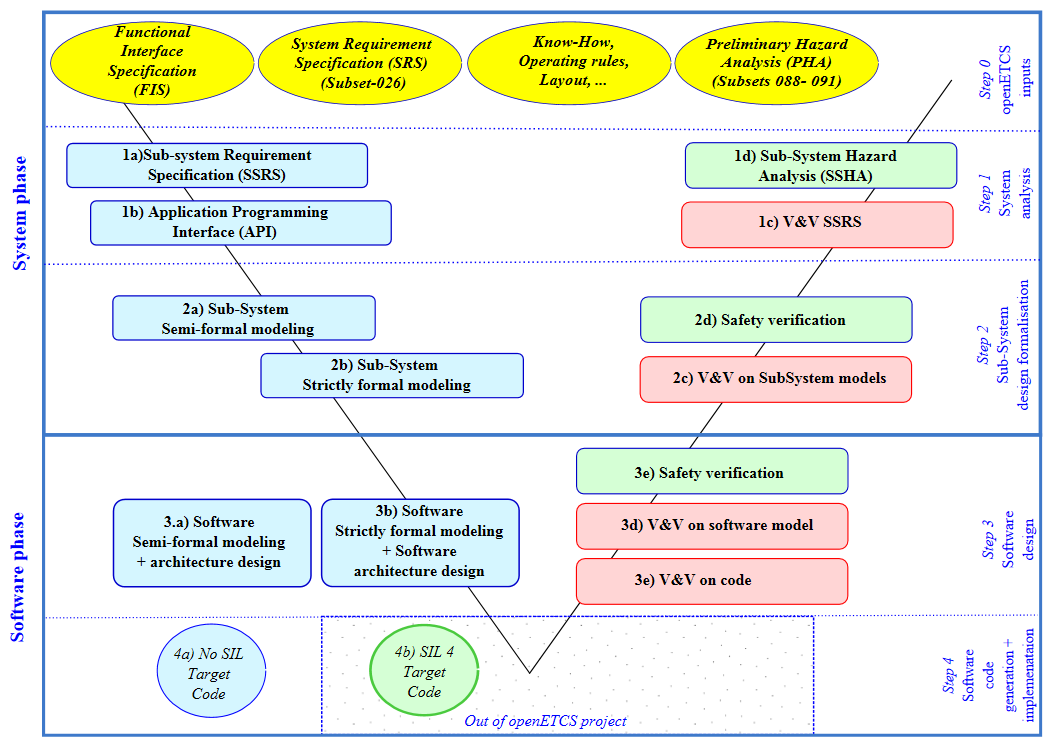
\includegraphics[width=.9\textwidth]{images/ProcessOpenETCS-BeM.png}
  \caption{openETCS Process (rough view)}
  \label{fig:openETCSProcess}
\end{figure}

According figure \ref{fig:openETCSProcess}, for which activities is the mean or tool suitable (see also \citep{D4.1} section 5.1.2 for more details) ?


\begin{tabular}{|l | c | c | c | c|}
\hline
& \textcolor{green}{Author} & \textcolor{blue}{Assessor 1} & \textcolor{magenta}{Assessor 2} & Total \\
\hline 
1c SSRS Verification & & & &  \\
\hline
1c SSRS Validation & & & &  \\
\hline
2c SFM Verification & & & &  \\
\hline
2c SFM Validation & & & &  \\
\hline
3d SW-SFM Verification & & & &  \\
\hline
3d SW-SFM Validation & & & &  \\
\hline
3d SW-FFM Verification & & & &  \\
\hline
3d SW-FFM Validation & & & &  \\
\hline
3e Code Verification & & & &  \\
\hline
3e Code Validation & & & &  \\
\hline
\end{tabular}


\subsection{Methods and tools}

Which kind of methods is proposed (see also \citep{D4.1} section 5.3) ?



\begin{tabular}{|l | c | c | c | c|}
\hline
& \textcolor{green}{Author} & \textcolor{blue}{Assessor 1} & \textcolor{magenta}{Assessor 2} & Total \\
\hline 
Reviews & & & &  \\
\hline
Inspections & & & &  \\
\hline
Software Architecture Analysis Method & & & &  \\
\hline
Architecture Tradeoff Analysis Method & & & &  \\
\hline
Model-Based System Integration Testing & & & &  \\
\hline
Model-Based Testing of Generated High-Level Code & & & &  \\
\hline
Abstract Interpretation & & & &  \\
\hline
Deductive Verification & & & &  \\
\hline
Model Checking & & & &  \\
\hline
Correct by Construction Formal Methods & & & &  \\
\hline
Verification with Formal Methods & & & &  \\
\hline
\end{tabular}

\begin{comment}
MPD : Todo

The sequel is let as an example is this early version.

Criteria to discuss here are those which concerns means and tools for VnV

7.7.3
Testing
R-WP2/D2.6-01-036 The SFM shall be simulable in debug mode (step-by-step), allowing inspec-
tion of states, variables and I/O.
R-WP2/D2.6-01-037 The environment shall be emulated by high level construction of the inputs.
Justification. “High level” means that it will not be necessary to define bitwise the inputs
at each cycle. On the contrary, some automation will be available to define the behavior
of the inputs.
R-WP2/D2.6-02-080 The environment shall be emulated by construction of the inputs compliant
to SUBSET-026.
R-WP2/D2.6-02-081 The tool chain shall allow time-based test cases.
R-WP2/D2.6-01-038 The tool chain shall allow to write, execute and store test cases and use
cases for the SFM.
R-WP2/D2.6-02-082 Version management will allow to map test cases version to the SFM, the
FFM and source code versions.
R-WP2/D2.6-02-083 The tool chain shall allow to generate test cases for the SFM, the FFM and
source code from a test model.
R-WP2/D2.6-02-083.01 The test model is independant from the tested model.
Justification. The test model can be either a model of the environment, or a model of the
same subsystem that is being tested, but in both cases this test model must be completely
independant from the tested model.
R-WP2/D2.6-02-084 The tool chain shall allow to write, execute and store test sequences com-
bining multiple test cases for the SFM, the FFM and source code.


\end{comment}




\section{Means and tools for safety activities support}
\label{sec:safety}

Criteria of this section are defined according \citep{D4.2.a}.

\subsection{Safety activities}

Which safety design activities is covered by the mean or tool (see \citep{D4.2.a} section 1.2) ?

\begin{tabular}{|l | c | c | c | c|}
\hline
& \textcolor{green}{Author} & \textcolor{blue}{Assessor 1} & \textcolor{magenta}{Assessor 2} & Total \\
\hline 
Preliminary Hazard Analysis & & & &  \\
\hline
Establish Safety Plan & & & & \\
\hline
System Hazard and Risk Analysis & & & & \\
\hline
Risk Assessment & & & & \\
\hline
Specification of System Safety Requirements & & & &  \\
\hline
Define Safety Related Functional Requirements & & & & \\
\hline
Specify Sub-System and Component & & & & \\
Safety requirements & & & & \\
\hline
Implement Safety Plan & & & & \\
\hline
Verify System, Sub-System and Component & & & &  \\
Safety requirements & & & &  \\
\hline
Validate System Safety Requirements & & & & \\
\hline
Establish Safety Case & & & & \\
\hline
\end{tabular}


\subsection{Input Artifacts}

Which artifacts are used as input of the mean or tool (see \citep{D4.2.a} section 1.4) ? 


\begin{tabular}{|l | c | c | c | c|}
\hline
& \textcolor{green}{Author} & \textcolor{blue}{Assessor 1} & \textcolor{magenta}{Assessor 2} & Total \\
\hline 
Safety Requirement & & & &  \\
\hline
Hazard log & & & & \\
\hline
Safety Plan & & & & \\
\hline
Safety Case & & & & \\
\hline
Code Safety Backlog & & & &  \\
\hline
Detailed Model Safety Backlog & & & & \\
\hline
High Level Safety Backlog & & & & \\
\hline
\end{tabular}



\subsection{Output Artifacts}

Which artifacts are used as output of the mean or tool (see \citep{D4.2.a} section 1.4) ? 


\begin{tabular}{|l | c | c | c | c|}
\hline
& \textcolor{green}{Author} & \textcolor{blue}{Assessor 1} & \textcolor{magenta}{Assessor 2} & Total \\
\hline 
Safety Requirement & & & &  \\
\hline
Hazard log & & & & \\
\hline
Safety Plan & & & & \\
\hline
Safety Case & & & & \\
\hline
Code Safety Backlog & & & &  \\
\hline
Detailed Model Safety Backlog & & & & \\
\hline
High Level Safety Backlog & & & & \\
\hline
\end{tabular}

\subsection{Expressiveness}


Which degree of formalisation is given to the artifacts by mean or tools (see \citep{D4.2.a} section 1.4) ? 


\begin{tabular}{|l | c | c | c | c|}
\hline
& \textcolor{green}{Author} & \textcolor{blue}{Assessor 1} & \textcolor{magenta}{Assessor 2} & Total \\
\hline 
Informal & & & &  \\
\hline
Semi-Formal & & & & \\
\hline
Formal & & & & \\
\hline
\end{tabular}


\subsection{Other criteria}
According to \citep{D4.2.a} section 2.2, provide some complement on the mean or tool:


\begin{tabular}{|l | c | c | c | c|}
\hline
& \textcolor{green}{Author} & \textcolor{blue}{Assessor 1} & \textcolor{magenta}{Assessor 2} & Total \\
\hline 
Top-Down approach  & & & &  \\
\hline
Bottom-up approach & & & & \\
\hline
Database capability & & & & \\
\hline
Database query ability & & & & \\
\hline
Safety requirement VnV & & & & \\
\hline
Traceability & & & & \\
\hline
Generation of documentation & & & & \\
\hline
\end{tabular}


\section{Means and tools for data, function and requirement management}
\label{sec:management}


\begin{comment}
MPD : Todo

The sequel is let as an example is this early version.

Criteria to discuss here are those which concerns management of repository for data, function and requirements
\end{comment}



\begin{tabular}{|l | c | c | c | c|}
\hline
& \textcolor{green}{Author} & \textcolor{blue}{Assessor 1} & \textcolor{magenta}{Assessor 2} & Total \\
\hline 
System Analysis & & & &  \\
\hline
Sub-system formal design & & & & \\
\hline
Software design & & & & \\
\hline
Software code generation & & & & \\
\hline
\end{tabular}


\section{Means and tools for model transformation and code generation}
\label{sec:transformation}


\begin{comment}
MPD : Todo

The sequel is let as an example is this early version.

Criteria to discuss here are those which concerns means and tools to model transformation and code generation
\end{comment}


\begin{tabular}{|l | c | c | c | c|}
\hline
& \textcolor{green}{Author} & \textcolor{blue}{Assessor 1} & \textcolor{magenta}{Assessor 2} & Total \\
\hline 
System Analysis & & & &  \\
\hline
Sub-system formal design & & & & \\
\hline
Software design & & & & \\
\hline
Software code generation & & & & \\
\hline
\end{tabular}
